\clearpage
\section[\textsc{implicit functions}]{IMPLICIT FUNCTIONS}
Consider the function $f\colon{}\F{R}^2\to \F{R}$ defined by $f(x, y) = x^2 + y^2 -1$. If 
we choose $(a, b)$ with $f(a, b) = 0$ and $a\neq 1, -1$, there are  (Figure \ref{Fig 2-4}) open 
interval $A$ containing $a$ and $B$ containing $b$ with the following property:
if $x\in A$, there is a unique $y\in B$ with $f(x, y) = 0$. We can therefore define 
a function $g\colon{}A\to \F{R}$ by the condition $g(x)\in B$ and $f(x, g(x)) = 0$ (if $b>0$,
as indicate in \figref{Fig 2-4}, then $g(x) = \sqrt{1-x^2}$). For the function $f$ we are considering
there is an interval $B_1$ containing $b_1$ such that $g(a, b_1)=0$. There will also be 
an interval $B_1$ such that, when $x\in A$, we have $f(x, g_1(x)) = 0$ for a unique $g_1(x)\in b_1$ 
(here $g_1(x) = -\sqrt{1-x^2}$). Both $g$ and $g_1$ are differentiable. These functions are 
said to be defined \textbf{implicitly}\index{Function!implicitly defined}%
\indexseealso{Function!implicitly defined}{Implicit Function Theorem}\index{Implicitly defined function} by the equation $f(x, y) = 0$.

\begin{figure}[!htb]
  \centering
  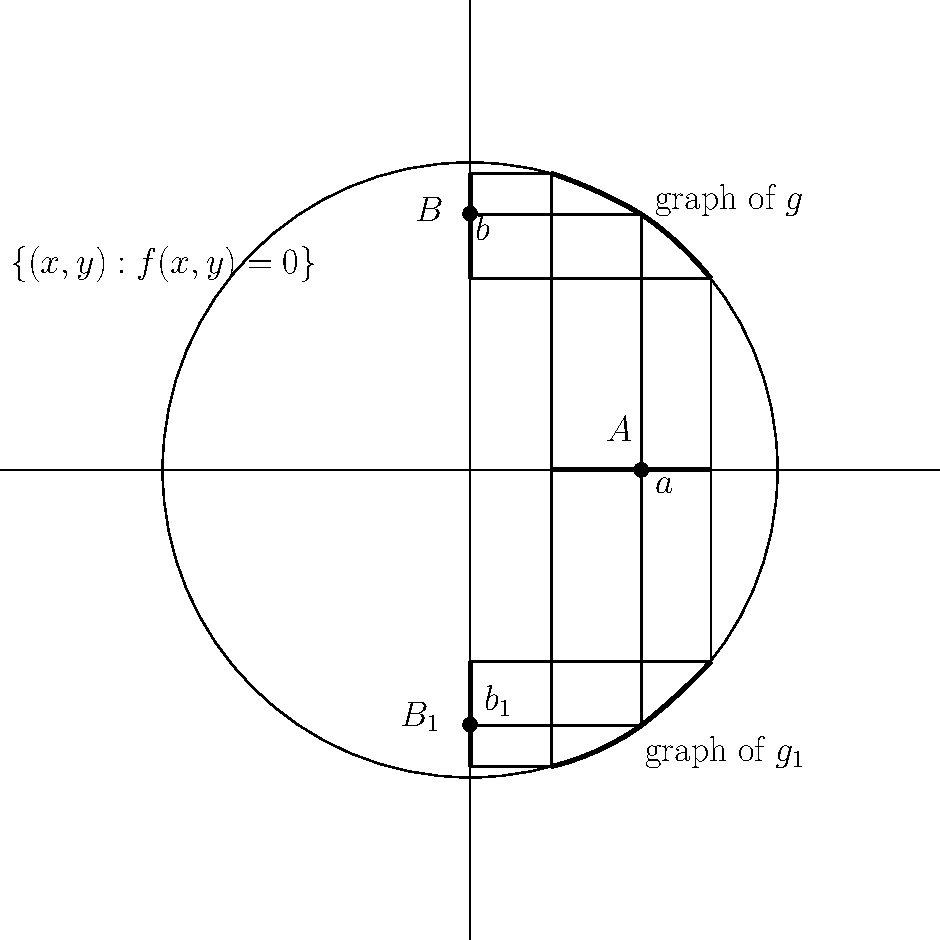
\includegraphics[width=.75\linewidth]{./pics/Fig2-4.pdf}
  \caption{}
  \label{Fig 2-4}
\end{figure}

If we choose $a = 1$ or $-1$ it is impossible to find any such
function $g$ defined in an open interval containing $a$.
We would like a simple criterion for deciding when, in general,
such a function can be found. More generally we may ask
the following: If $f\colon{}\F{R}^n \times \F{R}\to \F{R}$ and 
$f(a^1,\cdots,a^n, b) = 0$, when can we find, for each 
$(x^1,\cdots ,x^n)$ near $(a^1,\cdots,a^n)$,
a unique $y$ near $b$ such that $f(x^1,\cdots,x^n,y) = 0$ ? Even
more generally, we can ask about the possibility of solving
$m$ equations, depending upon parameters $x^1,\cdots,x^n$, in $m$
unknowns: If
\begin{align*}
    f_i:\F{R}^n\times \F{R}^m \to \F{R}\qquad i=1, \cdots, m
\end{align*}
and
\begin{align*}
    f_i:(a^1, \cdots, a^n, b^1, \cdots, b^m) = 0\qquad i=1, \cdots, m,
\end{align*} 
when can we find, for each $(x^1,\cdots,x^n)$ near $(a^1,\cdots,a^n)$ a unique 
$(y^1,\cdots,y^n)$ near $(b^1,\cdots,b^n)$ which satisfies $f_i(x^1,\cdots,x^n, y^1,\cdots,y^n)$?
The answer is provided by 
\begin{theorem}[Implicit Function Theorem]\index{Implicit Function Theorem}
    Suppose $f_i:\F{R}^n\times \F{R}^m$ is continuously differentiable in an open set
    containing $(a,b)$ and $f(a,b) = 0$. Let M be the $m\times m$ matrix
    \begin{align*}
        (\R{D}_{n+1}f^i(a, b))\qquad 1\le i,j\le m.
    \end{align*}

    If  $\det M \neq 0$, there is an open set $A \subset \F{R}^n$ containing $a$ 
    and an open set $B \subset \F{R}^m$ containing $b$, with the following property: for
    each $x \in A$ there is a unique $g(x) \in B$ such that $f(x,g(x)) = 0$.
    The function $g$ is differentiable.
\end{theorem}

\begin{proof}
    Define $f_i:\F{R}^n\times \F{R}^m\times R^m$ by $F(x, y) = (x, f(x, y))$. Then 
    $\det F'(a, b) = \det M\neq 0$. By Theorem 2-11 there is an open set $W\subset \F{R}^n\times \F{R}^m$
    containing $F(a, b)=(a, 0)$ and an open set in $\F{R}^n\times \F{R}^m$ containing $(a, b)$, which
    we may take to be the form $A\times B$, such that $f\colon{}A\times B\to W$ has a differentiable inverse 
    $h\colon{}W\to A\times B$. Clearly $h$ is of the form $h(x, y) = (x, k(x, y))$ for some differentiable 
    function $k$ (since $F$ is of this form). Let $\pi: \F{R}^n\times \F{R}^m \to \F{R}^m$ be defined 
    by $\pi(x, y) = y$; then $\pi\circ F = f$. Therefore 
    \begin{align*}
        f(x, k(x,y)) 
        & = f\circ h(x, y) = (\pi\circ F)\circ h(x, y) \\
        & = \pi\circ (F\circ h)(x, y) = \pi(x, y) = y.
    \end{align*} 

    Thus $f(x, k(x, 0)) = 0$; in other words we can define $g(x) = k(x, 0)$.
\end{proof}

Since the function g is known to be differentiable, it is easy
to find its derivative. In fact, since $f^i(x,g(x)) = 0$, taking $\R{D}_j$
of both sides gives 
\begin{align*}
    0 = \R{D}_jf^i(x, g(x)) + \sum_{\alpha=1}^{m}{\R{D}_{n+\alpha}f^i(x, g(x))\cdot \R{D}_jg^\alpha(x)} \\
    i,j = 1, \cdots, m.
\end{align*}

Since $\det M\neq 0$, these equations can be solved for $\R{D}_jg^\alpha(x)$.
The answer will depend on the various $\R{D}_jf^i(x, g(x))$, and therefore 
on $g(x)$. This is unavoidable, since the fucntion $g$ is not unique.
Reconsidering the function $f\colon{}\F{R}^2\to \F{R}$ defined by $f(x, y) = x^2 + y^2 -1$, we 
note that two possible functions satisfying $f(x, g(x)) = 0$ are $g(x) = -\sqrt{1-x^2}$ and 
$g(x) = \sqrt{1-x^2}$. Differentiable $f(x, g(x)) = 0$ gives 
\begin{align*}
    \R{D}_1f(x, g(x)) + \R{D}_2(x, g(x))\cdot g'(x) = 0,
\end{align*}
or 
\begin{align*}
  2x + 2g(x)\cdot g'(x) & = 0\\
  g'(x) &  = -x/g(x),
\end{align*}
which is indeed the case for either 
$g(x)\hspace*{-3pt} =\hspace*{-3pt} \sqrt{1-x}$ or $g(x)\hspace*{-3pt} =\hspace*{-3pt} -\sqrt{1-x^2}$.
A generalization of the argument for Theorem 2-12 can be given, which will be important in Chapter 5. 

\begin{theorem}
    Let $f\colon{}\F{R}^n\to \F{R}^p$ be continuously differentiable in an open set 
    containing $a$, where $p\le n$. If $f(a)=0$ and the $p\times n$ matirx $(\R{D}_jf^i(a))$ has 
    rank $p$, then there is an open set $A\subset \F{R}^n$ containing $a$ and a differentiable 
    function $h\colon{}A\to \F{R}^n$ with differentiable inverse such that 
    \begin{align*}
        f\circ h(x^1, \dots, x^n) = (x^{n-p+1}, \cdots, x^n).
    \end{align*}  
\end{theorem}

\begin{proof}
    We can consider $f$ as a function $f\colon{}\F{R}^{n-p}\times \F{R}^p\to \F{R}^p$.
    If $\det M\neq 0$, then $M$ is the $p\times p$ matrix $(\R{D}_{n-p-j}f^i(a)), 1\le i,j\le p$,
    then we are precisely in the situation considered in the proof of Theorem 2-12, and as we 
    showed in that proof, there is $h$ such that $f\circ h(x^1, \cdots, x^n) = (x^{n-p+1}, \cdots, x^n)$.
    
    In general, since $(\R{D}_jf^i(a))$ has rank $p$, there will be $j_1<\cdots<j_p$ such that the
    matirx $(\R{D}_jf^i(a)), 1\le i\le p, j=j_1, \cdots, j_p$ has non-zero determinant. If $g\colon{}\F{R}^n\to \F{R}^n$ 
    permutes the $x^j$ so that $g(x^1, \cdots, x^n) = (\cdots, x^{j_1}, \cdots, x^{j_p})$, then 
    $f\circ g$ is a function of the type already considered, so $((f\circ g)\circ k)(x^1,\cdots, x^n) = (x^{n-p+1}, \cdots, x^n)$ 
    for some $k$.  Let $h=g\circ k$.  
\end{proof}

\begin{problems}
    \problem{Use the implicit function theorem to re-do Problem 2-15(c).}
    \problem{Let $f\colon{}\F{R}\times \F{R}\to \F{R}$ be differentiable. For each $x\in \F{R}$ define 
        $g_x:\F{R}\to \F{R}$ by $g_z(y) = f(x, y)$. Suppose that for each $x$ there is a unique 
        $y$ with $g_x'(y) = 0$; Let $c(x)$ be this $y$.
        \begin{enumerate}[label={\upshape(\alph*)}]
            \item If $\R{D}_{2, 2}f(x, y)\neq 0$ for all $(x, y)$, show that $c$ is differentiable and 
                \begin{align*}
                    c'(x) = -\frac{\R{D}_{2,1}f(x, c(x))}{\R{D}_{2, 2}f(x, c(x))}.
                \end{align*}
                \textit{Hint:} $g_z'(y) = 0$ can be written $\R{D}_2f(x, y) = 0$.
            \item Show that if $c'(x) = 0$, then for some $y$ we have 
                \begin{align*}
                  \R{D}_{2,1}f(x, y) & = 0, \\
                  \R{D}_2f(x,y) & = 0.
                \end{align*}
            \item Let $f(x, y) = x(y\ln y - y) - y\ln x$, Find 
                \begin{align*}
                    \max_{\frac{1}{2}\le x\le 2}\big(\min_{\frac13\le y\le 1}f(x, y)\big).
                \end{align*}
        \end{enumerate}
        }
\end{problems}